\section{POSIX IO Overheads}
\label{sec:posix-overheads}

\begin{figure}[tb]
\centering
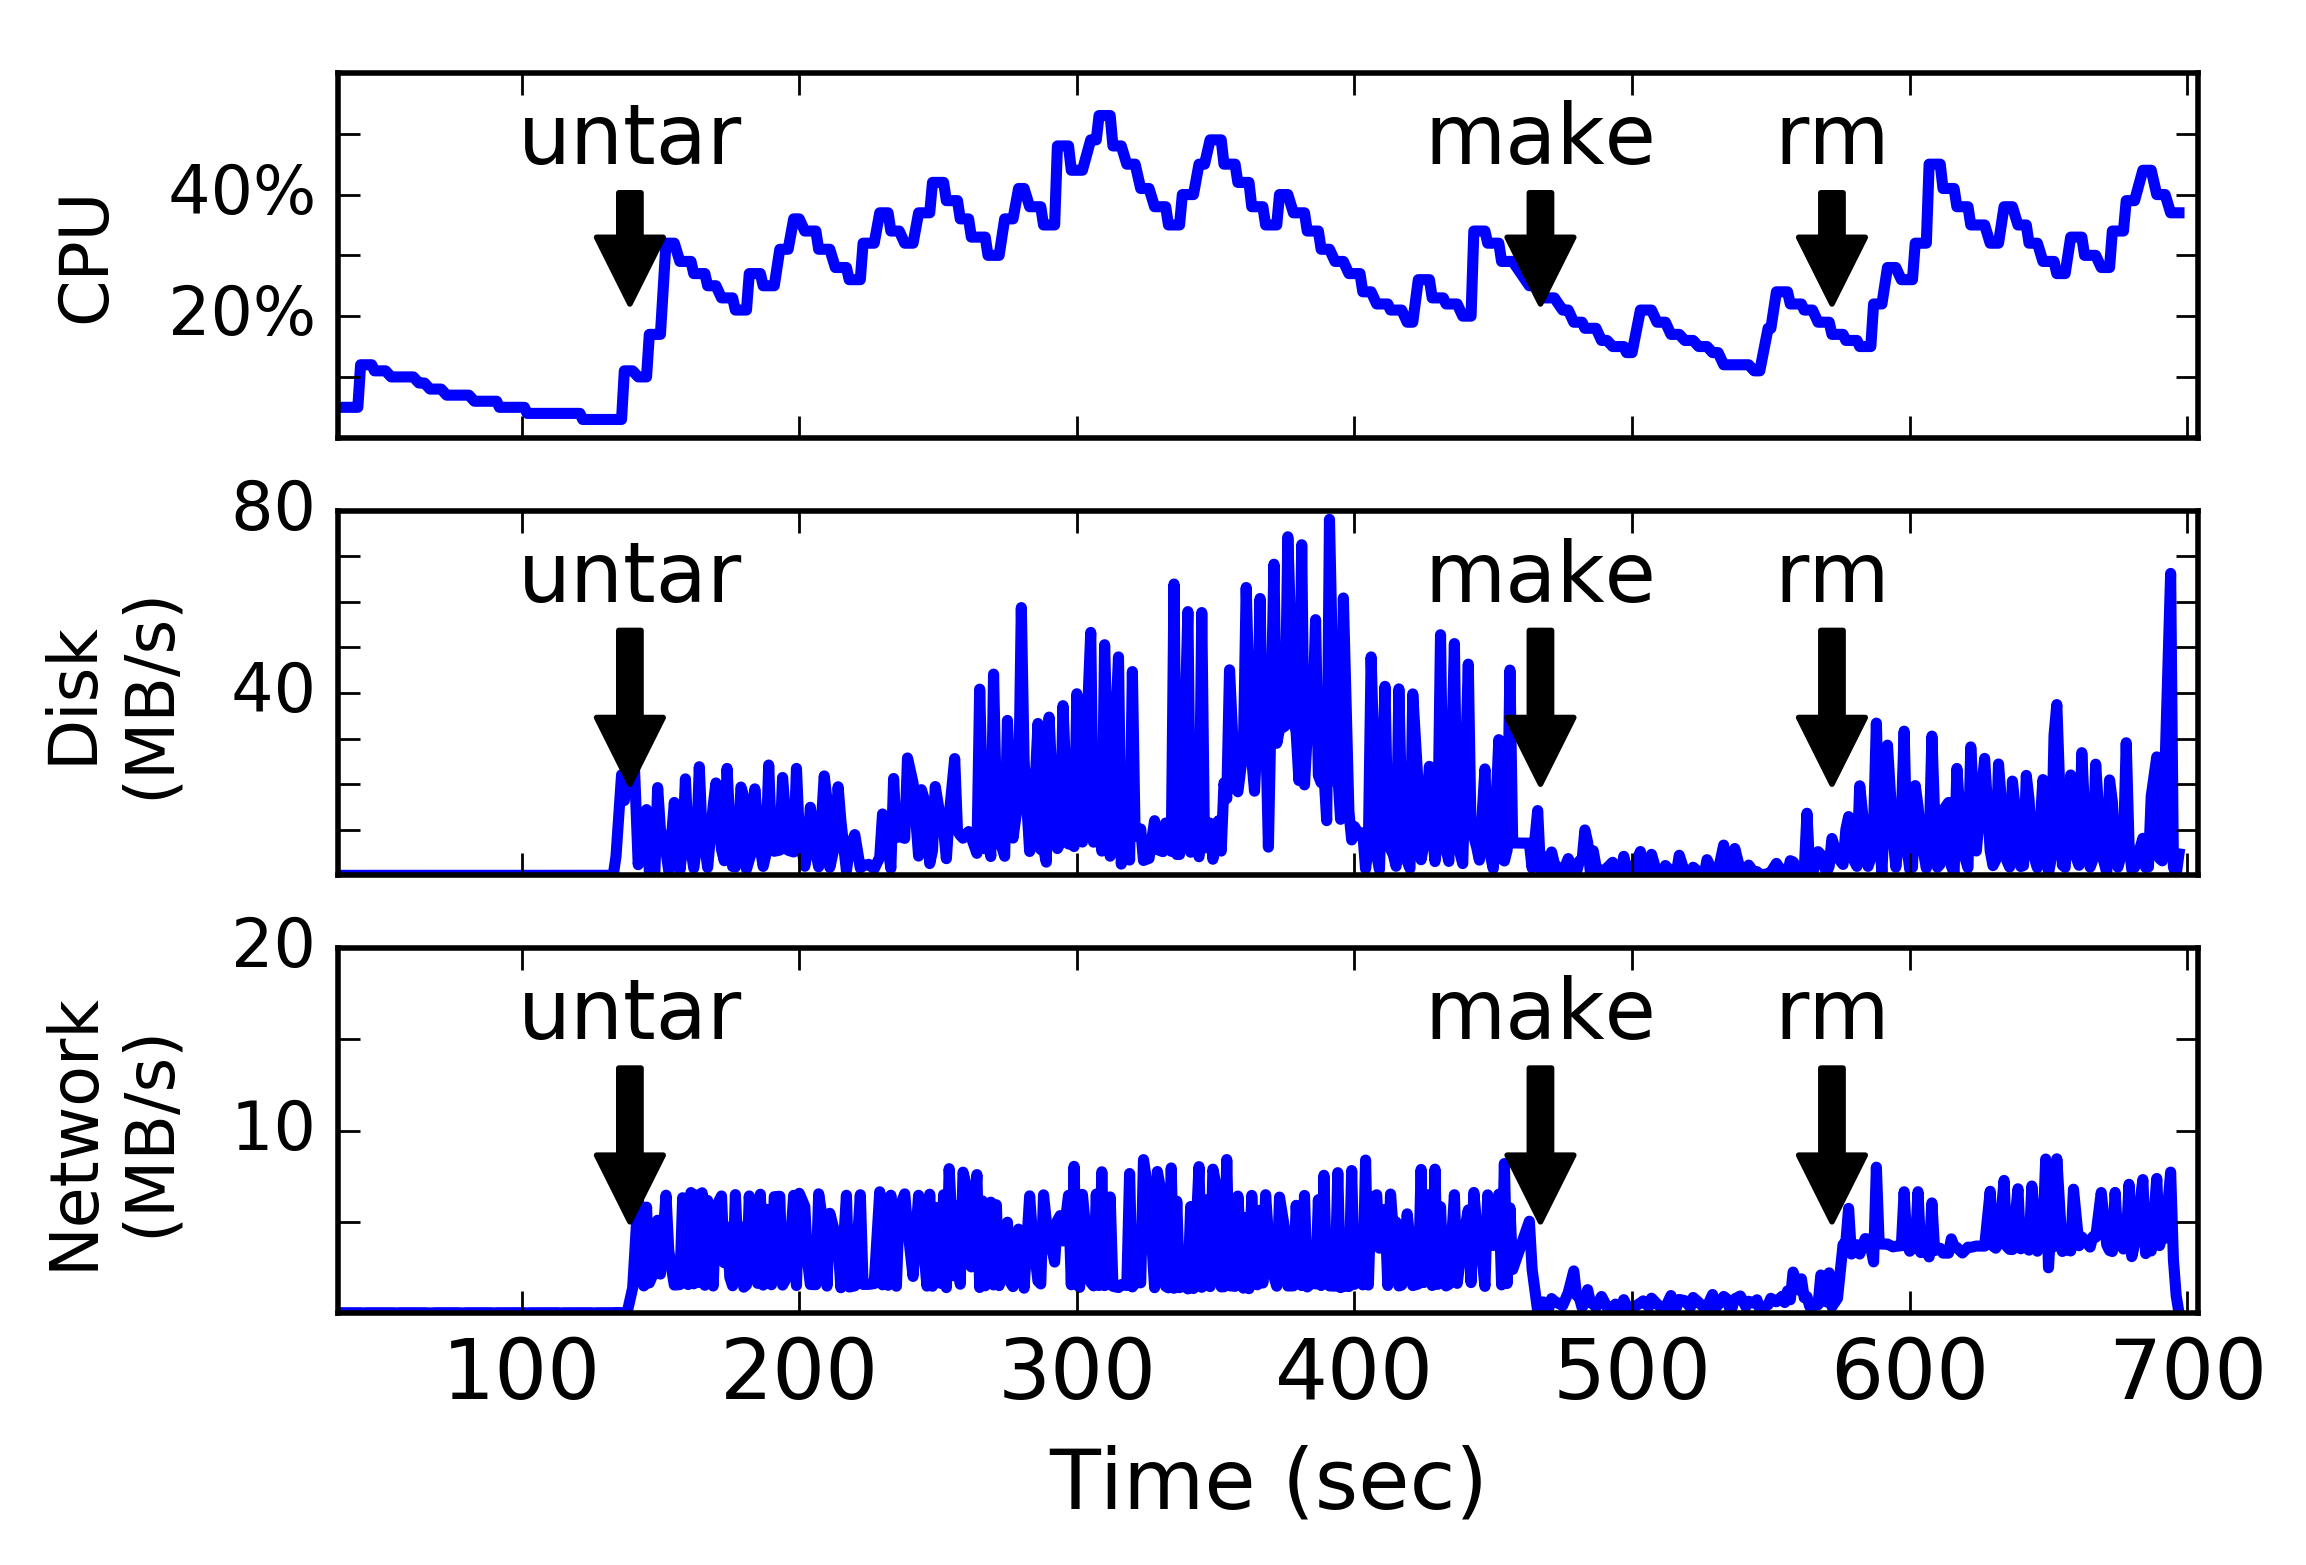
\includegraphics[width=1\linewidth]{./graphs/overhead-creates.png}

\caption{[\href{https://github.com/michaelsevilla/cudele-popper/blob/revision/experiments/baseline-compile/visualize/viz.ipynb}{source}]
Create-heavy workloads (such as \texttt{untar}) incur the highest disk,
network, and CPU utilization because of the consistency and durability demands
of CephFS.}\label{fig:overhead-creates}

\end{figure}

In our examination of the overheads of POSIX IO we benchmark and analyze
CephFS, the file system that uses Ceph's object store ({\it i.e.} RADOS) to
store its data and metadata. To show how the file system behaves under high
metadata load we use a create-heavy workload.  During this process we
discovered, based on the analysis and breakdown of costs, that durability and
consistency have high overhead but we urge the reader to keep in mind that this
file system is an implementation of one set of design decisions and our goal
here is to highlight the effect that those decisions have on performance.

Figure~\ref{fig:overhead-creates} shows the resource utilization of compiling
the Linux kernel in a CephFS mount.  The \texttt{untar} phase, which is
characterized by many creates, has the highest resource usage (combined CPU,
network, and disk) because of the number of RPCs needed for consistency and
durability. The RPCs are also serialized because the metadata server is single
threaded; although na\"{\i}ve, this design is common because of the complexity
of multi-threaded metadata
servers~\cite{konstantinos:pdsw2014-lustre-metadata}.  In this section, we
quantify the costs of consistency and durability in CephFS.  At the end of each
subsection we compare the approach to ``decoupled namespaces", the technique in
related work that detaches subtrees from the global namespace to relax
consistency/durability guarantees. 

\subsection{Durability}
\label{sec:durability}

\begin{figure*}[t]
  \centering
  \begin{subfigure}[b]{.3\linewidth}
      \centering
      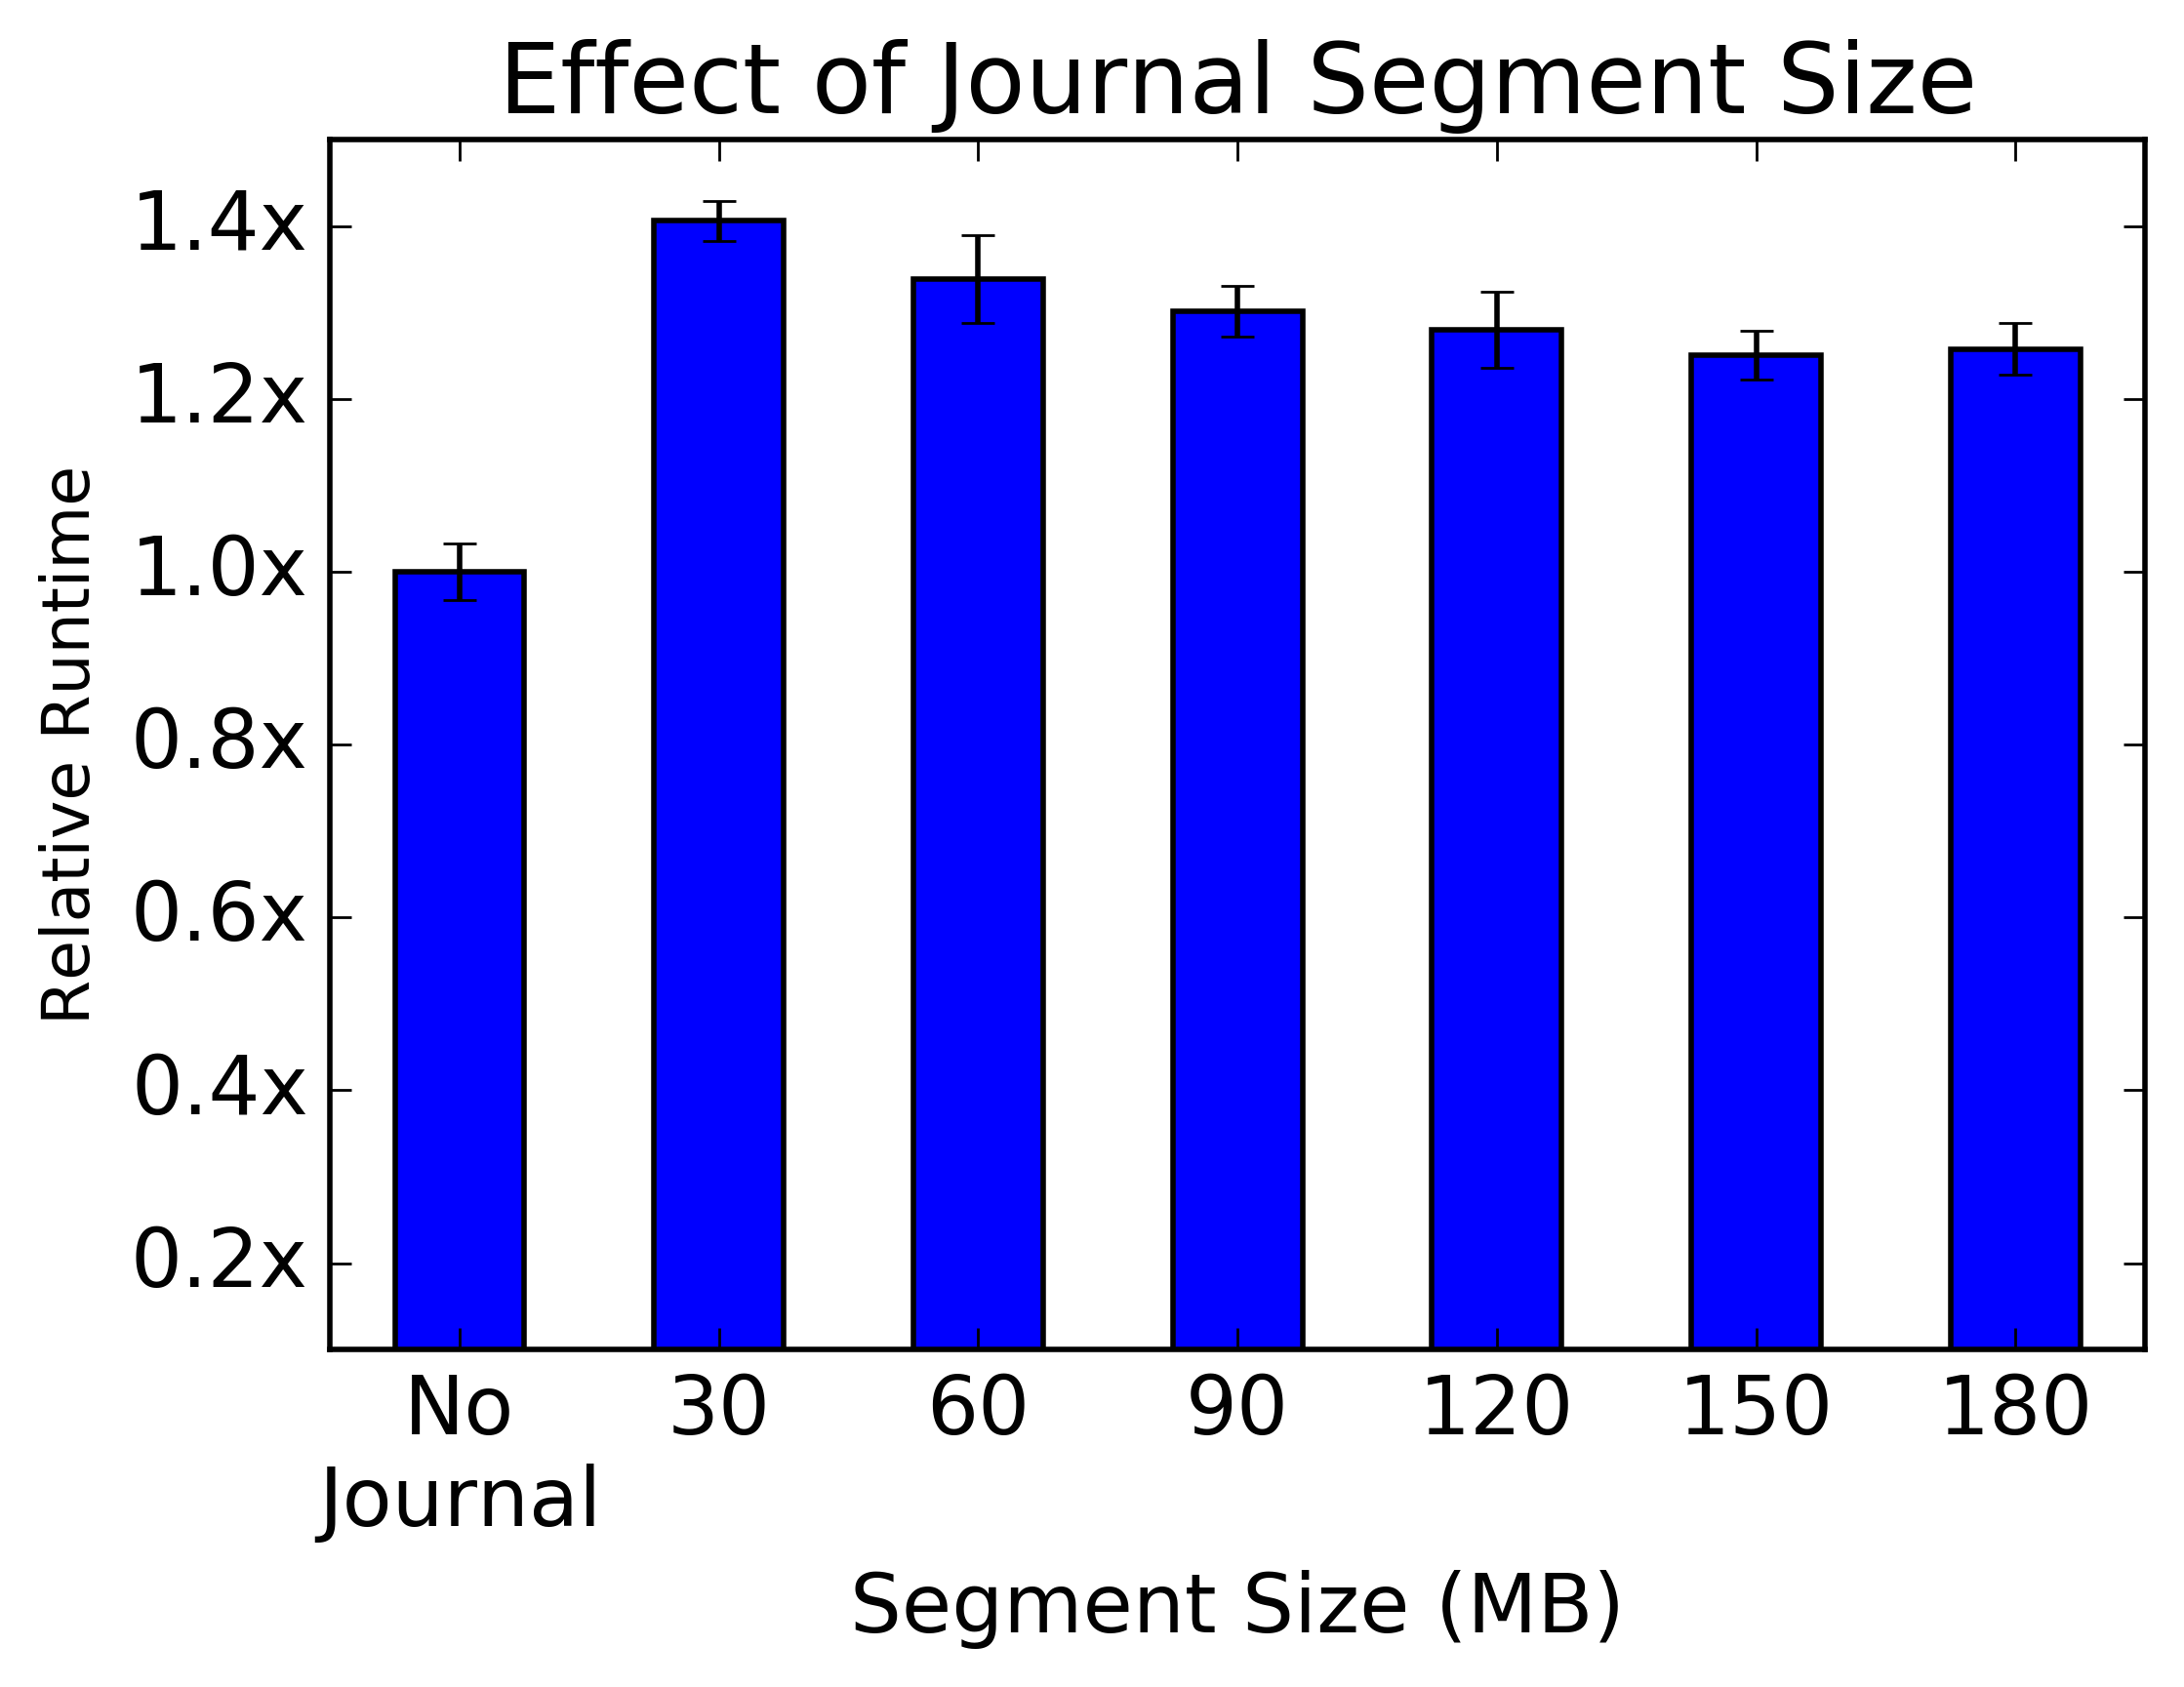
\includegraphics[width=0.95\linewidth]{graphs/slowdown-journal.png}
      \caption{[\href{https://github.com/michaelsevilla/cudele-popper/blob/revision/experiments/baseline-durability/visualize/viz.ipynb}{source}]
      Effect of Journal} \label{fig:overhead-a}
  \end{subfigure}
  \begin{subfigure}[b]{.3\linewidth}
      \centering
      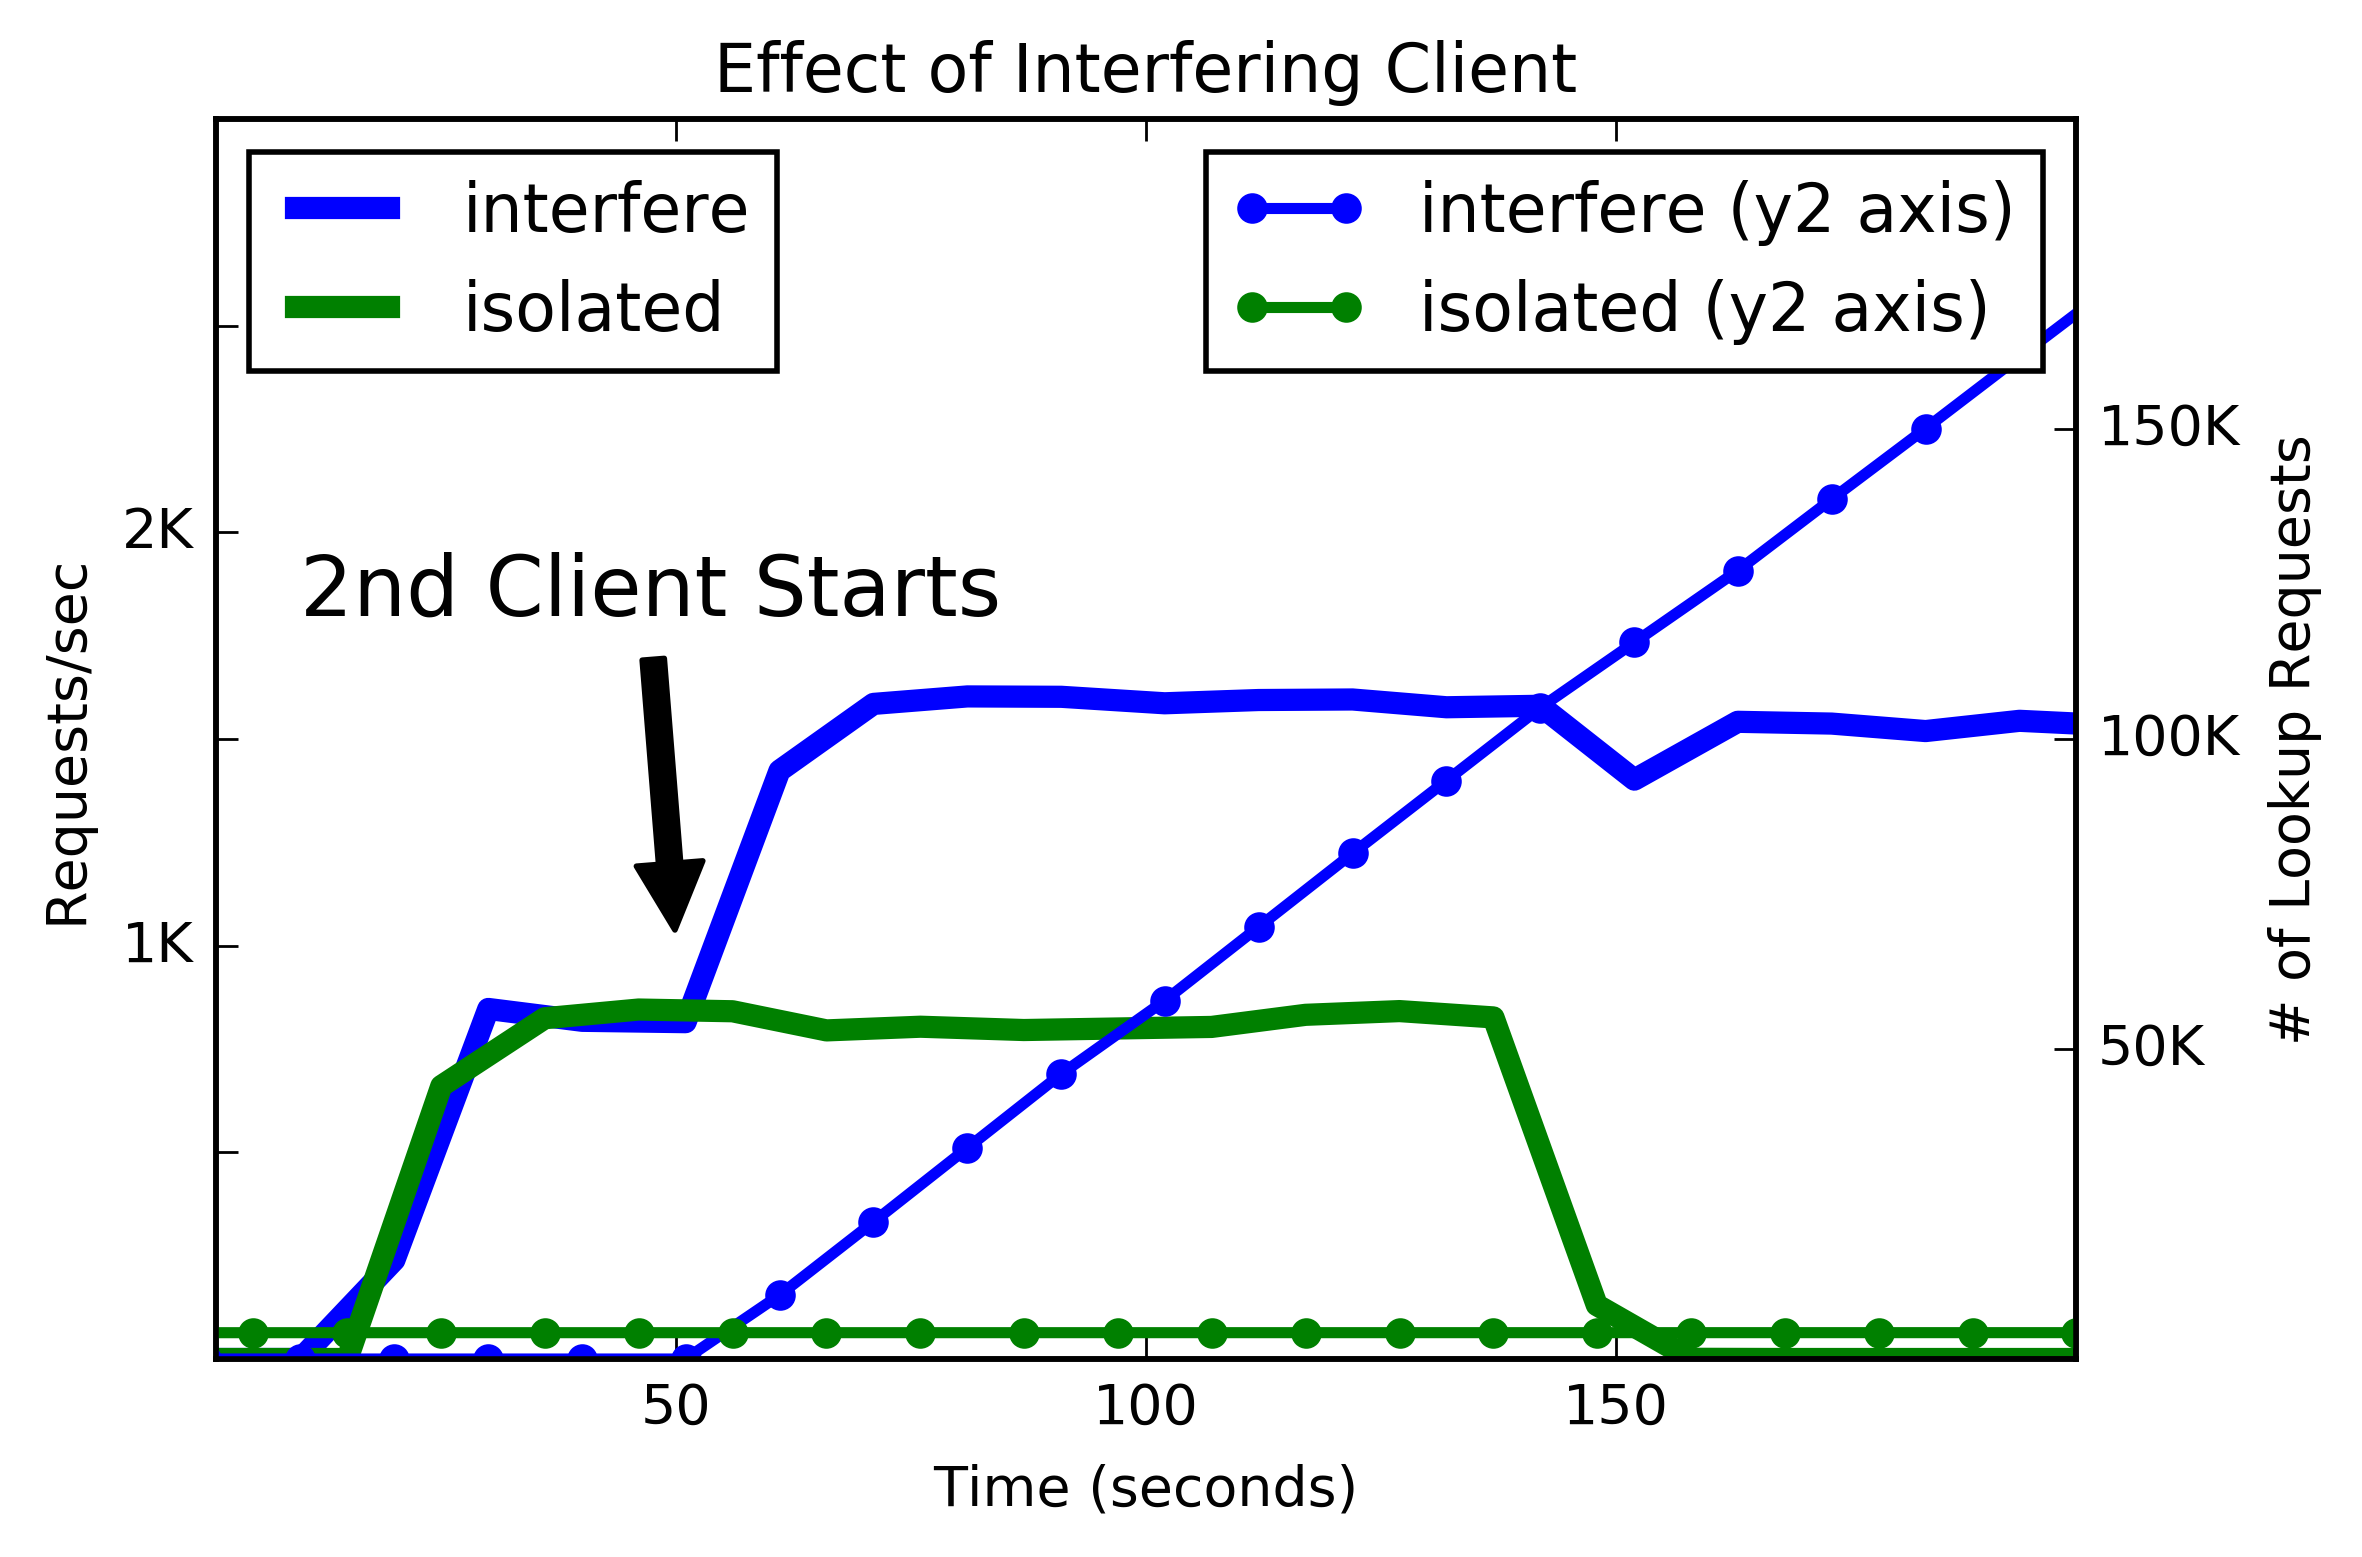
\includegraphics[width=1.1\linewidth]{graphs/behavior-interfere.png}
      \caption{[\href{https://github.com/michaelsevilla/cudele-popper/blob/revision/experiments/baseline-interfere/visualize/viz.ipynb}{source}]
      Interference increases RPCs}
      \label{fig:overhead-b}
  \end{subfigure}
  \begin{subfigure}[b]{.3\linewidth}
      \centering
      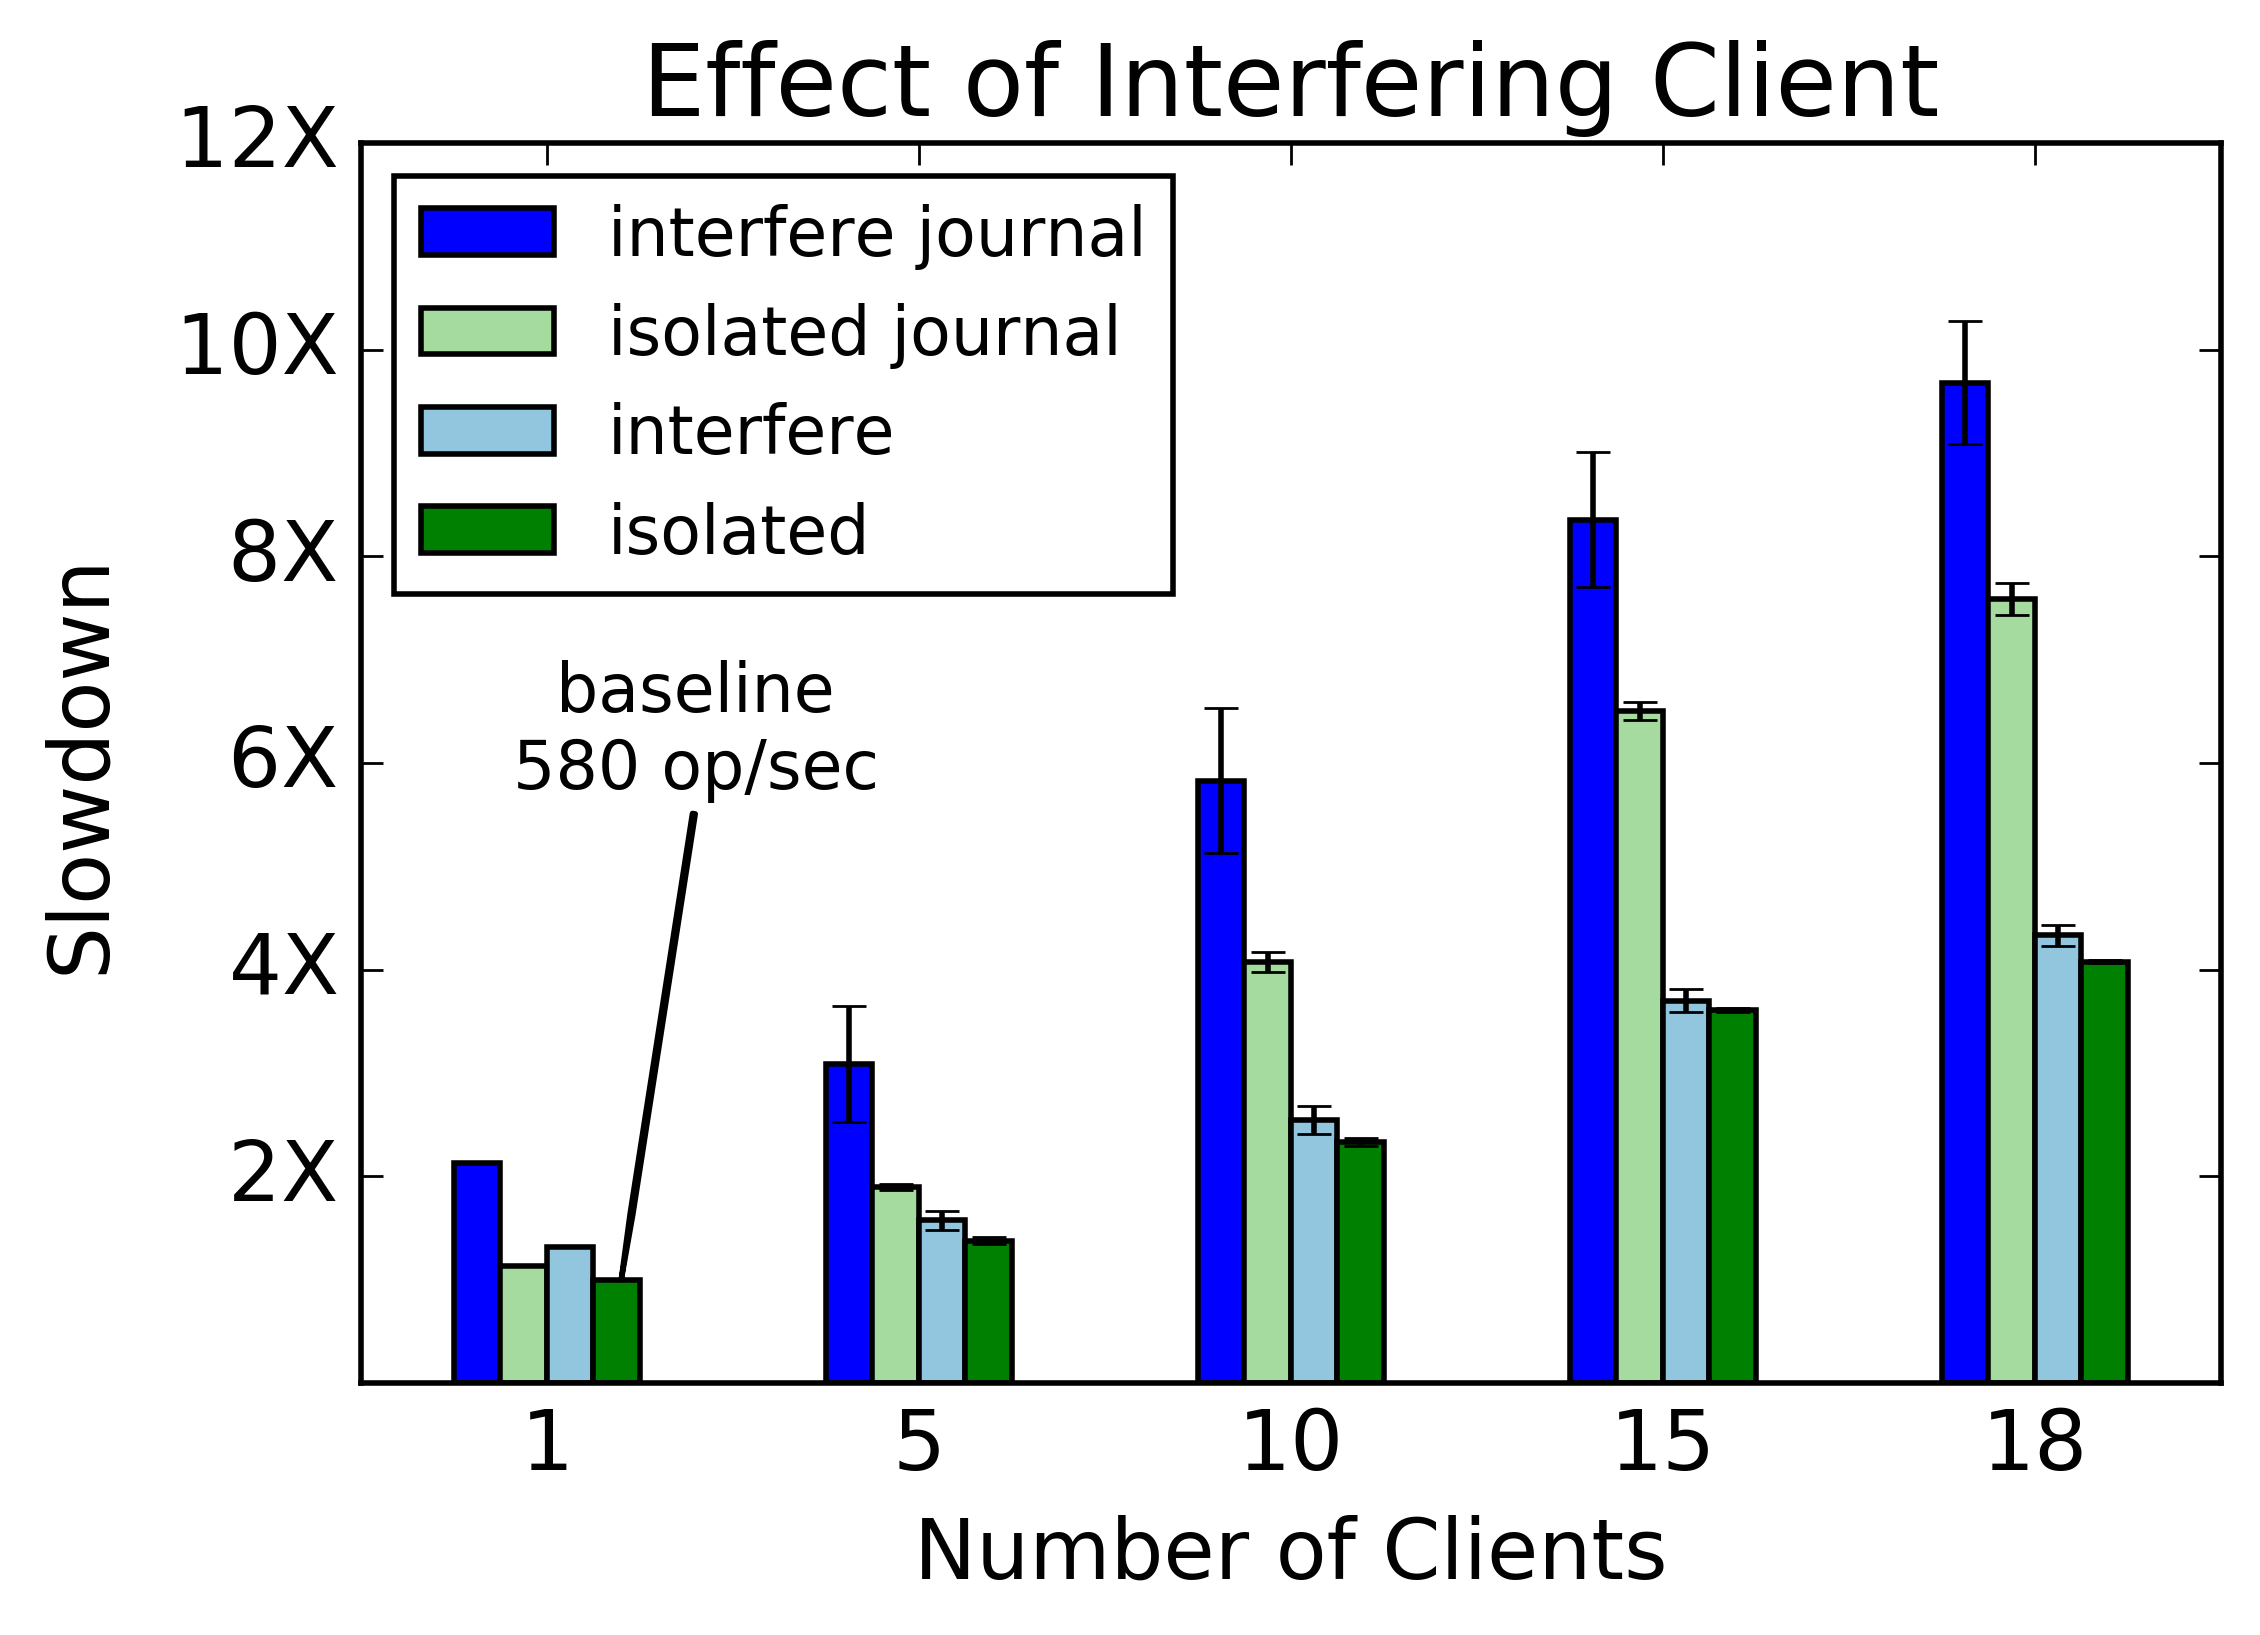
\includegraphics[width=1\linewidth]{graphs/slowdown-interfere-scale.png}
      \caption{[\href{https://github.com/michaelsevilla/cudele-popper/blob/revision/experiments/baseline-creates/visualize/viz.ipynb}{source}]
      Interference hurts variability}
      \label{fig:overhead-c}
  \end{subfigure}
  \caption{ The overhead of durability and strong consistency in CephFS.  (a)
  shows the effect of different journal segment sizes, normalized to a setup
  without a journal (``No Journal").  The journal is streamed into the object
  store for fault tolerance. (b) and (c) show that when a second client
  ``interferes", capabilities are revoked and metadata servers do more work.
  \label{fig:overhead}}
\end{figure*}

% what is durability
While durability is not specified by POSIX IO, users expect that files they
create or modify survive failures.  We define three types of durability:
global, local, and none.  Global durability means that the client or server can
fail at any time and metadata will not be lost because it is ``safe" ({\it
i.e.} striped or replicated across a cluster). Local durability means that
metadata can be lost if the client or server stays down after a failure. None
means that metadata is volatile and that the system provides no guarantees when
clients or servers fail.  None is different than local durability because
regardless of the type of failure, metadata will be lost when components die in a
None configuration.

% - sequential IO, trim redundant operations
\textbf{CephFS Design}: A journal of metadata updates that streams into the
resilient object store. Similar to LFS~\cite{rosenblum:acm1992-LFS} and
WAFL~\cite{hitz:wtec1994-WAFL} the metadata journal is designed to be large
(on the order of MBs) which ensures (1) sequential writes into the object store
and (2) the ability for daemons to trim redundant or irrelevant journal
entries.  The journal is striped over objects where multiple journal updates
can reside on the same object. There are two tunables for controlling the
journal: the segment size and the number of segments that can be written in
parallel. Unless the journal saturates memory or CPU resources, larger values
for these tunables results in better performance.

% purpose of the journal
In addition to the metadata journal, CephFS also represents metadata in RADOS
as a metadata store, where directories and their file inodes are stored as
objects.  The metadata server applies the updates in the journal to the
metadata store when the journal reaches a certain size. The metadata store is
optimized for recovery ({\it i.e.} reading) while the metadata journal is
write-optimized.

%\begin{figure}[tb] \centering
%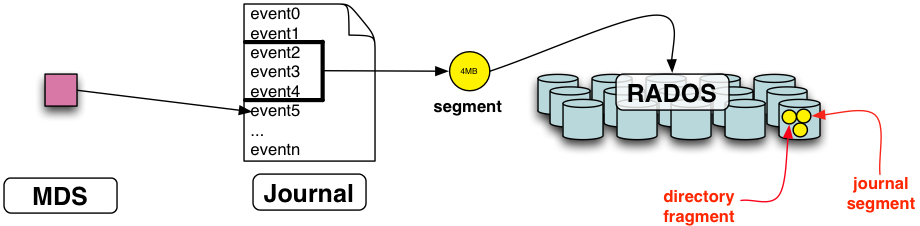
\includegraphics[width=1\linewidth]{./figures/journal.png} 
%\caption{CephFS has two views of the file system namespace: a journal of
%metadata updates and a metadata store. For fault tolerance, they are stored in
%the object store as segments and fragments, respectively.
%\label{fig:journal}}
%\end{figure}

% Effects on performance
Figure~\ref{fig:overhead-a} shows the effect of journaling of with different
segment sizes; the larger the segment size the bigger that the writes into the
object store are. The trade-off for better performance is memory consumption
because larger segments take up more space for buffering. When journaling is
on, the metadata server periodically stops serving requests to flush ({\it
i.e.} apply journal updates) to the metadata store.  The journal overhead is
sufficient enough to slow down metadata throughput but not so much as to
overwhelm the bandwidth of the object store. 

\textbf{Comparison to decoupled namespaces}: For BatchFS, if a client fails
when it is writing to the local log-structured merge tree (implemented as an
SSTable~\cite{ren:atc2013-tablefs}) then unwritten metadata operations are
lost. For DeltaFS, if the client fails then, on restart, the computation does
the work again -- since the snapshots of the namespace are never globally
consistent and there is no ground truth.  On the server side, BatchFS and
DeltaFS use IndexFS~\cite{ren:sc2014-indexfs}. IndexFS writes metadata to
SSTables, which initially reside in memory but are later flushed to the
underlying distributed file system.

\subsection{Strong Consistency}
\label{sec:strong-consistency}

Access to metadata in a POSIX IO-compliant file system is strongly consistent, so
reads and writes to the same inode or directory are globally ordered.  The
synchronization and serialization machinery needed to ensure that all clients
see the same state has high overhead.

\textbf{CephFS Design}: Capabilities keep metadata strongly
consistent. To reduce the number of RPCs needed for consistency, clients can
obtain capabilities for reading and writing inodes, as well as caching reads,
buffering writes, changing the file size, and performing lazy IO.

% inode cache - reduces RPCs (lookups for create, readdirs for stats)
To keep track of the read caching and write buffering capabilities, the clients
and metadata servers agree on the state of each inode using an inode cache.  If
a client has the directory inode cached it can do metadata writes ({\it e.g.},
create) with a single RPC. If the client is not caching the directory inode
then it must do an extra RPC to determine if the file exists.  Unless the
client immediately reads all the inodes in the cache ({\it i.e.} \texttt{ls
-alR}), the inode cache is less useful for create-heavy workloads.

% benefits PROBLEM -- IS THIS THE METADATA PROTOCOL OR JUST THE OVERLOADEDNESS?
The benefits of caching the directory inode when creating files is shown in
Figure~\ref{fig:overhead-b}. The colors show the behavior of the client for two
different runs.  If only one client is creating files in a directory
(``isolated" curve on \(y1\) axis) then that client can lookup the existence of
new files locally before issuing a create request to the metadata server. If
another client starts creating files in the same directory then the directory
inode transitions out of read caching and the first client must send
\texttt{lookup()}s to the metadata server (``interfere" curve on \(y2\) axis).
These extra requests increase the throughput of the ``interfere" curve on the
\(y1\) axis because the metadata server can handle the extra load but
performance suffers.  This degradation is shown in Figure~\ref{fig:overhead-c},
where we scale the number of clients and show the slowdown of the slowest
client.  The results are normalized to a single isolated client without a
metadata server journal and the error bars are the standard deviations of all
client runtimes.  For the ``interfere" bars, each client creates files in
private directories and at 30 seconds we launch another process that creates
files in those directories. 18 is the maximum number of clients the metadata
server can handle for this metadata-intensive workload; at higher client load,
the metadata server complains about laggy and unresponsive requests.

% TODO: what is the cost of trimming the cache?
% TODO: does CephFS still cache inodes when I turn off caching? Why is still keeping inodes in memory? Gah!

\textbf{Comparison to decoupled namespaces}: Decoupled namespaces
merge batches of metadata operations into the global namespaces when the job
completes.  In BatchFS the merge is delayed by the application using an API to
switch between asynchronous and synchronous mode. The merge itself is explicitly
managed by the application but future work looks at more automated
methodologies. In DeltaFS snapshots of the metadata subtrees stays on the client
machines; there is no ground truth and consistent namespaces are constructed
and resolved at application read time or when a 3rd party system ({\it e.g.},
middleware, scheduler, etc.) needs a view of the metadata. As a result, all the
overheads of maintaining consistency that we showed above are delayed until the
merge phase.
